En esta sección se detallan todas las tecnologías utilizadas a lo largo del desarrollo del proyecto, desde lenguajes y sistemas internos del motor de desarrollo hasta software concreto de diseño audiovisual y de gestión del proyecto. También se tratan las metodologías utilizadas en los meses de desarrollo tanto para la organización de tareas como de comunicación y supervisión con el tutor.

\section{Motor de Videojuegos: Unity 6 \cite{unity_engine}}
Para el desarrollo del prototipo se ha seleccionado la última iteración del motor de videojuegos de Unity Technologies, conocida comercialmente como \textbf{Unity 6} (versión de compilación específica \texttt{6000.3.8f1}) (ver Figura~\ref{fig:unity6}).

\begin{figure}[H]
    \centering
    
\includegraphics[width=0.25\textwidth]{pages/img/Unity6.png}
    \caption{Logotipo de Unity6.}
    \label{fig:unity6}
\end{figure}

\subsection{Justificación Técnica y Elección del Motor}
La elección de Unity 6 frente a otras alternativas del mercado se fundamenta en criterios de eficiencia de desarrollo, arquitectura interna y viabilidad para proyectos independientes:

\begin{itemize}
    \item \textbf{Especialización en entornos bidimensionales:} A diferencia de otros motores optimizados prioritariamente para el renderizado fotorrealista en tres dimensiones, Unity 6 integra un ecosistema nativo avanzado para el desarrollo 2D y 2.5D. Herramientas como el sistema de \textit{Tilemaps} o el empaquetador de gráficos optimizan la creación de escenarios modulares y la gestión de recursos visuales sin sobrecargar el rendimiento del sistema.
    
    \item \textbf{Ecosistema y documentación técnica:} La API de Unity destaca por ser una de las más documentadas y estandarizadas de la industria. Disponer de un marco de soporte tan amplio mitiga los riesgos técnicos durante el desarrollo, facilitando la resolución de problemas lógicos y la implementación de patrones de diseño de software extendidos.
    
    \item \textbf{Modelo de licenciamiento:} El acceso a la licencia \textit{Unity Personal} permite el uso íntegro de las capacidades del motor de forma gratuita para proyectos académicos o de investigación sin presupuesto inicial, eliminando barreras económicas y garantizando la viabilidad del proyecto.

    \item \textbf{Curva de experiencia previa:} El uso de este motor de videojuegos a lo largo de la formación académica del grado garantiza un dominio técnico avanzado de su interfaz y arquitectura. Optar por una tecnología familiar reduce drásticamente el tiempo invertido en la fase de adaptación y aprendizaje básico, lo que se traduce en una mayor eficiencia operativa, soltura en la resolución de problemas y optimización de los plazos de entrega del proyecto.
\end{itemize}

\subsection{Rol en el Proyecto}
Unity 6 opera como el núcleo central del videojuego, coordinando los subsistemas principales que componen la experiencia interactiva y garantizando la cohesión entre la lógica de software y la representación multimedia. Su rol se distribuye en las siguientes áreas fundamentales:

\begin{itemize}
    \item \textbf{Subsistema de Físicas Dinámicas (Box2D):} El motor gestiona de manera nativa la simulación de fuerzas, gravedad y colisiones aplicadas sobre los elementos mecánicos del juego. Este motor bidimensional se emplea tanto para calcular el movimiento preciso del personaje en entornos de plataformas como para realizar comprobaciones de proximidad y detecciones espaciales en tiempo real entre las distintas entidades del mundo virtual.
    
    \item \textbf{Canalización de Renderizado (Universal Render Pipeline - URP):} Se ha utilizado la tubería de renderizado ligero URP configurada específicamente para entornos bidimensionales. Esta tecnología permite procesar de manera eficiente la estética visual del juego, gestionando el comportamiento de las cámaras, la ordenación de las capas de renderizado (\textit{Sorting Layers}) y el procesado de imágenes con un bajo consumo de recursos de hardware.
    
    \item \textbf{Controlador de Animaciones (Mecanim):} El sistema nativo de animación gestiona los ciclos visuales de las entidades mediante máquinas de estado jerárquicas. Este componente traduce las variables lógicas controladas por código en transiciones visuales fluidas, aislando la lógica pura del juego de la representación gráfica del personaje.
    
    \item \textbf{Administración del Ciclo de Vida y Gestión de Escenas:} El motor actúa como el gestor de memoria principal del proyecto, controlando la carga y descarga asíncrona de los diferentes niveles, mundos y menús interactivos. Esta característica es fundamental para asegurar la persistencia de los datos de control y garantizar transiciones fluidas entre los distintos estados del juego sin provocar caídas en el rendimiento.
    
    \item \textbf{Sistema de Interfaz de Usuario (UI):} Unity coordina la capa de presentación gráfica superpuesta que comunica información crítica al jugador (como indicadores de estado, inventarios o menús de navegación). El motor gestiona de forma nativa la escalabilidad de estos elementos según la resolución de la pantalla y procesa los eventos de interacción del usuario de manera aislada al bucle lógico del juego.
\end{itemize}

\subsection{Pipeline de Trabajo e Integración de Recursos}
El flujo de desarrollo dentro de Unity 6 se ha estructurado como un proceso sistemático para asimilar la naturaleza multigénero del proyecto. El motor actúa como un entorno unificado donde confluyen el diseño modular de niveles y la arquitectura de software a través de tres fases clave:

\begin{enumerate}
    \item \textbf{Procesamiento y Estructuración de Activos Visuales:} Los recursos gráficos bidimensionales importados se configuran mediante perfiles específicos sin compresión para preservar la fidelidad del estilo artístico. El uso del \textit{Sprite Editor} integrado permite segmentar las hojas de recursos y definir de manera precisa los puntos de pivote físicos de las entidades, garantizando que las detecciones de suelo y las alineaciones espaciales sean coherentes con la lógica de control.
    
    \item \textbf{Construcción Modular de Escenarios (\textit{Tilemaps}):} La arquitectura de los niveles se diseña de forma eficiente mediante el sistema nativo de rejillas y paletas de celdas. Esta metodología permite pintar los entornos de manera modular y automatizar la generación de colisiones físicas mediante componentes como \textit{Tilemap Collider 2D} y \textit{Composite Collider 2D}. Este flujo agiliza el diseño de los escenarios de los diferentes mundos y optimiza el rendimiento del motor al fusionar múltiples geometrías de colisión individuales en una única malla unificada.
    
    \item \textbf{Vinculación Lógica y Parametrización en el Inspector:} El nexo entre el código en C\# y el entorno visual se realiza a través de la interfaz del Inspector de Unity. Al exponer y serializar variables críticas de los scripts (como fuerzas de salto, velocidades de movimiento o tiempos de reutilización), el motor permite modificar estos atributos en tiempo de ejecución. Esta característica resulta fundamental para calibrar y equilibrar las distintas mecánicas y físicas exigidas por cada género de videojuego sin necesidad de reescribir ni recompilar el código fuente constantemente.
\end{enumerate}



\section{Lenguaje de Programación: C\# \cite{csharp_spec}}
Toda la lógica de juego, la simulación física personalizada, la inteligencia artificial de las entidades y el sistema de guardado y carga han sido implementados en \textbf{C\#} (C-Sharp) (ver Figura~\ref{fig:marioworld}). C\# es un lenguaje de programación multiparadigma moderno, fuertemente tipado y administrado por el entorno de desarrollo de Unity, actuando como el lenguaje vehicular para estructurar las mecánicas interactivas del videojuego.

\begin{figure}[H]
    \centering
    
\includegraphics[width=0.25\textwidth]{pages/img/CSharp.png}
    \caption{Logotipo de C\#.}
    \label{fig:csharp}
\end{figure}

\subsection{Justificación Técnica y Arquitectura de Software}
La selección de C\# está ligada al uso de Unity como motor de juego principal, al ser su lenguaje de programación estándar nativo. C\# proporciona una sintaxis robusta basada en la programación orientada a objetos que permite gestionar de forma eficiente sistemas de juego complejos, ofreciendo un equilibrio óptimo entre velocidad de desarrollo y rendimiento en tiempo de ejecución.:

\begin{itemize}
    \item \textbf{Gestión automatizada de memoria (Garbage Collector):} A diferencia de lenguajes de bajo nivel como C++, C\# opera sobre un entorno administrado que cuenta con un recolector de basura. Este componente libera automáticamente la memoria de los objetos dinámicos que dejan de ser referenciados por el juego, previniendo fugas de memoria (\textit{memory leaks}) y garantizando la estabilidad de la aplicación sin exigir una gestión manual de punteros.
    
    \item \textbf{Paradigma Orientado a Objetos (POO):} El lenguaje proporciona un soporte robusto para la implementación de principios de diseño orientado a objetos como la herencia y el polimorfismo. Esto resulta fundamental para abordar la naturaleza de un proyecto que combina múltiples géneros, permitiendo estructurar plantillas de comportamiento genéricas para las entidades y extenderlas en componentes especializados, reduciendo la redundancia y facilitando el mantenimiento del código fuente.
    
    \item \textbf{Desacoplamiento modular y delegados:} C\# facilita la creación de arquitecturas desacopladas mediante el uso de eventos y delegados. Esto permite separar la lógica de detección física del jugador de la respuesta de los elementos interactivos del entorno (como cajas, interfaces o portales), logrando que los sistemas se comuniquen entre sí de manera limpia y sin dependencias directas entre componentes.
\end{itemize}

\subsection{Rol en el Proyecto y Mecanismos Avanzados}
El lenguaje se ha empleado para programar las reglas y comportamientos del videojuego, coordinando la lógica abstracta a través de los siguientes mecanismos del entorno:

\begin{itemize}
    \item \textbf{Gestión del Ciclo de Vida del Motor:} C\# permite interactuar directamente con el bucle de ejecución del motor. De esta forma, el código coordina de manera ordenada la sincronización de las entradas del jugador, la actualización periódica de la lógica de los enemigos y el procesamiento de la simulación física de forma independiente a la tasa de fotogramas del dispositivo.
    
    \item \textbf{Serialización de Datos:} C\# proporciona las herramientas necesarias para traducir estructuras de datos complejas cargadas en la memoria activa del juego a formatos de almacenamiento estandarizados. Esto permite guardar y recuperar de forma estructurada el estado del inventario, los coleccionables y el progreso del jugador en el almacenamiento físico del sistema operativo.
\end{itemize}

\subsection{Pipeline de Trabajo (Flujo de Desarrollo)}
El ciclo de ingeniería de software con C\# sigue un proceso cerrado de implementación y verificación técnica dentro del entorno de desarrollo:

\begin{enumerate}
    \item \textbf{Programación de Componentes:} Se desarrollan scripts lógicos que heredan de las clases base del motor, lo que permite acoplarlos directamente a los elementos visuales y físicos del entorno de desarrollo interactivo.
    
    \item \textbf{Depuración y Trazabilidad de Errores:} El flujo de trabajo aprovecha la integración directa del código con las herramientas de diagnóstico del entorno de desarrollo integrado (IDE). Esto permite monitorizar el flujo de la lógica, examinar el estado de las variables lógicas en tiempo real e insertar puntos de interrupción (\textit{breakpoints}) para localizar fallos lógicos durante las fases de prueba.
\end{enumerate}

\section{Entorno de Desarrollo Integrado (IDE): Visual Studio \cite{visual_studio}}

Para la escritura, edición y depuración de todo el código fuente en C\#, se ha seleccionado el entorno de desarrollo integrado \textbf{Microsoft Visual Studio} (en su edición \textit{Community}) (ver Figura~\ref{fig:visual}).

\subsection{Justificación Técnica y Elección del IDE}
La elección de Visual Studio frente a otros editores de código ligero (como Visual Studio Code o Notepad++) responde a criterios de robustez técnica e integración nativa con el motor de videojuegos:

\begin{figure}[H]
    \centering
    
\includegraphics[width=0.25\textwidth]{pages/img/VisualStudio.png}
    \caption{Logotipo de Visual Studio.}
    \label{fig:visual}
\end{figure}
\begin{itemize}

    \item \textbf{Integración nativa con Unity:} Visual Studio cuenta con herramientas integradas específicas para Unity (\textit{Game Development with Unity workload}). Esto permite la sincronización automática de la solución del proyecto, facilitando que el IDE reconozca instantáneamente todas las clases, métodos e interfaces propias de la API del motor.
    
    \item \textbf{IntelliSense y análisis de código estático:} El motor de autocompletado inteligente ayuda a reducir errores de sintaxis y tipografía en tiempo de escritura. Además, el análisis estático advierte sobre posibles problemas de rendimiento específicos de Unity (como el uso ineficiente de búsquedas de componentes repetitivas o llamadas de físicas incorrectas) antes de compilar el software.
    
    \item \textbf{Licencia comunitaria gratuita:} La versión \textit{Community} ofrece todas las capacidades profesionales de depuración y refactorización de código sin coste para entornos educativos y desarrolladores independientes, garantizando la viabilidad de la herramienta dentro del proyecto.
\end{itemize}

\subsection{Rol en el Proyecto}
Visual Studio opera como el espacio de trabajo principal de ingeniería de software del videojuego, cumpliendo los siguientes roles:
\begin{itemize}
    \item \textbf{Edición y Refactorización de Código:} Permite organizar la arquitectura de scripts y realizar refactorizaciones seguras (como renombrar clases o variables en múltiples archivos a la vez) sin romper las dependencias lógicas del juego.
    
    \item \textbf{Depuración activa (Debugging) mediante acoplamiento:} El IDE permite acoplar su proceso de ejecución al editor de Unity en tiempo real. Esto hace posible insertar puntos de interrupción (\textit{breakpoints}) en líneas específicas de código. Cuando el juego se ejecuta y alcanza esa línea, la ejecución se congela, permitiendo al desarrollador examinar el valor exacto de las variables en memoria física (útil para diagnosticar fallos en la IA de los enemigos o en el comportamiento del selector de niveles).
\end{itemize}

\subsection{Pipeline de Trabajo (Flujo de Integración)}
El flujo de trabajo entre Visual Studio y Unity se realiza a través de un puente bidireccional automático:
\begin{enumerate}
    \item \textbf{Apertura y sincronización:} Al hacer doble clic en cualquier script en la interfaz de Unity, el motor de videojuegos abre el archivo en Visual Studio, sincronizando las referencias del proyecto de C\#.
    \item \textbf{Compilación asíncrona:} Al guardar los cambios en Visual Studio, Unity detecta de manera asíncrona la actualización del archivo en disco y compila automáticamente las modificaciones, permitiendo probar los cambios en el editor de forma casi instantánea.
\end{enumerate}

\section{Cliente de Control de Versiones: GitHub Desktop \cite{git}}
Para la administración del sistema de control de versiones Git y la sincronización con el repositorio remoto alojado en la nube, se ha seleccionado el cliente gráfico oficial \textbf{GitHub Desktop} (ver Figura~\ref{fig:github}). La elección de esta herramienta se justifica por la familiaridad y experiencia previa adquirida con su interfaz a lo largo del grado, lo que garantizó una curva de aprendizaje nula y una mayor agilidad en el desarrollo diario.

\begin{figure}[H]
    \centering
    
\includegraphics[width=0.25\textwidth]{pages/img/GitHubDesktop.png}
    \caption{Logotipo de GitHub Desktop.}
    \label{fig:github}
\end{figure}

A pesar de tratarse de un proyecto individual, se ha implementado de forma rigurosa una metodología de trabajo basada en ramas (\textit{branching}) para garantizar la estabilidad del software. En el desarrollo de videojuegos, las escenas de Unity (\textit{.unity}) y los prefabs (\textit{.prefab}) son archivos estructurados en formato YAML que se corrompen con facilidad y son extremadamente difíciles de fusionar ante cualquier conflicto. 

El uso de ramas independientes ha actuado como un entorno de pruebas seguro (\textit{sandbox}): cada nueva característica compleja (como la inteligencia artificial o el sistema de menús de pausa) se desarrolló en su propia rama dedicada. De este modo, si una implementación experimental fallaba o corrompía la escena de trabajo, bastaba con descartar esa rama sin poner en riesgo la compilación principal y estable del videojuego, la cual permanecía a salvo en la rama \textit{main}. Además, este modelo facilita la trazabilidad del proyecto al asociar cada rama a una tarea específica del tablero de gestión.

\section{Soporte y Asistencia en el Desarrollo: Antigravity \cite{antigravity_ai}}
Como parte del conjunto de herramientas de desarrollo, se ha utilizado el asistente de inteligencia artificial \textit{Antigravity} (desarrollado por el equipo de Google DeepMind) (ver Figura~\ref{fig:antigravity}) para dar soporte en las tareas de programación y documentación técnica del proyecto. Su integración en el flujo de trabajo ha operado bajo la metodología de programación en pareja (\textit{Pair Programming}), sirviendo de apoyo técnico en tres áreas fundamentales:

\begin{itemize}
    \item \textbf{Depuración de Ciclos de Vida y Sincronía:} Asistencia en la resolución de condiciones de carrera en el orden de ejecución nativo de Unity.
    \item \textbf{Estructuración de Algoritmia Física y Matemática:} Soporte en el desarrollo y validación matemática de las ecuaciones de movimiento, tales como el cálculo de vectores o las parábolas físicas del personaje.
    \item \textbf{Auditoría de Arquitectura de Código:} Colaboración en la estructuración modular de los gestores globales del juego, facilitando la implementación de patrones de diseño limpios y el desacoplamiento de datos a través de \textit{ScriptableObjects}.
\end{itemize}

De esta forma, la herramienta ha funcionado como un recurso de consulta y refactorización que ha permitido optimizar los tiempos de desarrollo, facilitando que el alcance del proyecto se viera proyectado exponencialmente en pro de una mejor experiencia de usuario.

\begin{figure}[H]
    \centering
    
\includegraphics[width=0.5\textwidth]{pages/img/Antigravity.png}
    \caption{Logotipo de Google Antigravity.}
    \label{fig:antigravity}
\end{figure}

\section{Herramientas de Diseño Gráfico, Animación y Audio}

Para dar soporte a la creación de los recursos visuales, las interfaces y los efectos sonoros del videojuego, se han empleado diversas herramientas multimedia especializadas:

\begin{itemize}
    \item \textbf{Adobe Photoshop: \cite{photoshop}} Esta herramienta de edición y manipulación de gráficos rasterizados (\textit{bitmaps}) de alta resolución se ha utilizado para el desarrollo de la identidad visual del proyecto principal y de los subentornos interactivos de cada nivel. Asimismo, se ha empleado en la composición técnica de las imágenes de fondo y en la creación, maquetación y dimensionado de los elementos constitutivos de la interfaz de usuario (UI), garantizando una canalización limpia de texturas hacia Unity 6. La elección de este software se fundamenta en la experiencia previa consolidada a lo largo de la formación académica. Esta soltura técnica ha permitido simplificar la creación de interfaces complejas y optimizar los tiempos de preproducción gráfica, asegurando un acabado estético profesional que facilita la posterior integración modular dentro del motor de videojuegos (ver Figura~\ref{fig:photoshop}).
    
    \item \textbf{Piskel: \cite{piskel}} Se trata de un editor de gráficos bidimensionales especializado en la creación y animación de \textit{Pixel Art} en formato de hojas de sprites (\textit{sprite-sheets}). Dado que el núcleo técnico de este TFG se centra en la ingeniería de software, la arquitectura lógica y el diseño de mecánicas de juego, la gran mayoría de los activos visuales provienen de librerías y paquetes de recursos de uso libre. En este escenario, Piskel ha actuado como la herramienta clave para la homogenización artística: se ha empleado para reescalar imágenes, corregir la paleta de colores de los recursos externos para integrarlos bajo una misma identidad cromática y diseñar de forma manual ciertos sprites de personajes, elementos interactivos del escenario y componentes de la interfaz de usuario (UI) que el prototipo requería a medida (ver Figura~\ref{fig:piskel}).
    
    \item \textbf{Audacity: \cite{audacity}} Esta herramienta de edición y grabación de audio digital de código abierto se ha utilizado para la manipulación, limpieza y optimización del apartado acústico del videojuego, abarcando tanto los efectos de sonido (como disparos, impactos físicos o sonidos ambientales) como las pistas de música ambiental. Audacity ha permitido realizar de forma ágil tareas de procesamiento de audio esenciales para el rendimiento del juego, incluyendo la reducción de ruido de fondo, el recorte de silencios muertos en los clips y la normalización de volumen. Asimismo, se ha empleado para exportar el audio en formatos compatibles optimizados para Unity: formato \texttt{.wav} sin compresión para efectos de corta duración que requieren reproducción instantánea, y formatos comprimidos como \texttt{.mp3} u \texttt{.ogg} para pistas de larga duración para minimizar el consumo de memoria del sistema (ver Figura~\ref{fig:audacity}).
\end{itemize}

\begin{figure}[H]
    \centering
    % Subfigura izquierda (Space Invaders)
    \begin{subfigure}[b]{0.2\textwidth}
        \centering
        
\includegraphics[width=\textwidth]{pages/img/Photoshop.png}
        \caption{Logotipo de Photoshop.}
        \label{fig:photoshop}
    \end{subfigure}
    \hfill
    % Subfigura central (Pac-Man)
    \begin{subfigure}[b]{0.2\textwidth}
        \centering
        
\includegraphics[width=\textwidth]{pages/img/Piskel.png}
        \caption{Logotipo de Piskel.}
        \label{fig:piskel}
    \end{subfigure}
    \hfill% Subfigura derecha (Pac-Man)
    \begin{subfigure}[b]{0.3\textwidth}
        \centering
        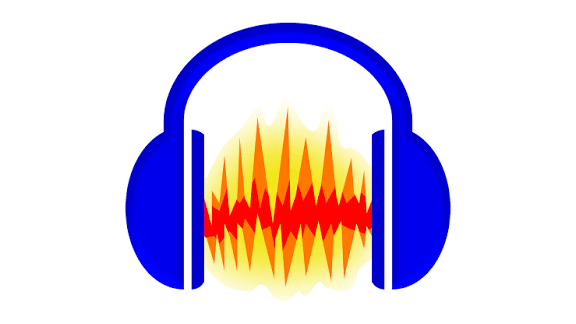
\includegraphics[width=\textwidth]{pages/img/Audacity.png}
        \caption{Logotipo de Audacity.}
        \label{fig:audacity}
    \end{subfigure}
    \caption{Herramientas de diseño y audio.}
    \label{fig:HerramientasDisenoAudio}
\end{figure}

\section{Herramientas de Gestión, Comunicación y Planificación}

Para la estructuración, el control temporal y la coordinación de las tutorías individuales durante la realización del TFG, se han utilizado los siguientes recursos organizativos:

\begin{itemize}
    \item \textbf{Microsoft Teams: \cite{ms_teams}} El canal de comunicación oficial utilizado para las reuniones periódicas con el tutor académico del TFG. A través de esta herramienta se han coordinado las entregas de avances de la memoria y las demostraciones funcionales del prototipo de cara a la tutorización y corrección del trabajo (ver Figura~\ref{fig:teams}).
    
    \item \textbf{Bloc de notas y Notas Manuales:} Utilizados en las fases de concepción rápida de ideas y durante las sesiones de prueba de juego (\textit{playtesting}). Han servido para registrar de forma ágil errores técnicos en caliente, realizar bocetos matemáticos de algoritmos y cálculo de físicas en diseño de niveles antes de codificarlos en C\# y listar tareas urgentes durante las sesiones frente al editor.
\end{itemize}

\begin{figure}[H]
    \centering
    
\includegraphics[width=0.4\textwidth]{pages/img/Teams.png}
    \caption{Logotipo de Microsoft Teams.}
    \label{fig:teams}
\end{figure}

\section{Metodología de Desarrollo Ágil Adaptada}
Al tratarse de un proyecto de desarrollo unipersonal, la implementación estricta de metodologías tradicionales o marcos de trabajo complejos (como Scrum puro) resultaba ineficiente y añadía una carga burocrática innecesaria. Por ello, a pesar de haber iniciado el proyecto mediante la mencionada metodología, se optó por una \textbf{metodología ágil adaptada}, priorizando la flexibilidad, la iteración rápida y la adaptación continua a los problemas de diseño que surgían durante la programación.

Para la organización de tareas, se sustituyeron los gestores de proyectos de gran escala por un sistema de \textbf{Product Backlog} simplificado y directo (mediante registros y notas personales). En este registro se centralizaron todas las ideas de diseño, la lista de mecánicas pendientes de implementar, los errores conocidos (\textit{bugs}) y las metas a corto plazo. Este enfoque minimalista permitió mantener el foco absoluto en el desarrollo del motor y en el diseño de niveles, evitando la fricción de gestionar plataformas externas complejas y que resultaban innecesarias para un proyecto unipersonal.

\section{Control de Progreso y Revisiones Iterativas}
Para garantizar que el proyecto cumpliera con los estándares académicos y los plazos de entrega, el desarrollo ágil se complementó con un sistema riguroso de control y revisión. 

Este seguimiento se materializó a través de dos vías de comunicación constante:

\begin{itemize}
    \item \textbf{Actualizaciones semanales (Dailies/Weeklies):} Reportes de estado mediante la plataforma Microsoft Teams, donde se documentaban los avances técnicos de la semana, los obstáculos encontrados en el código o en el diseño artístico, y los objetivos para los siguientes días.
    
    \item \textbf{Validación Académica (Sprint Reviews):} Reuniones bisemanales telemáticas y con el tutor del proyecto. Estas sesiones funcionaban como hitos de control donde se presentaban los prototipos jugables, se validaba el \textit{Game Feel} de las nuevas mecánicas y se reajustaban los objetivos del Documento de Diseño de Juego (GDD) en base a la retroalimentación recibida.
\end{itemize}

\section{Diseño Iterativo y Greyboxing}
El proceso de creación de los mundos de \textit{Reset} no fue lineal, sino fuertemente iterativo. Antes de invertir tiempo en la creación de los \textit{sprites} y la ilustración final en Pixel Art, los niveles se construyeron utilizando la técnica de \textbf{Greyboxing} \cite{greyboxing} (o \textit{Whiteboxing}). 

Esta metodología consistió en prototipar los escenarios en Unity utilizando formas geométricas básicas (bloques de colisión grises) para testear exclusivamente las mecánicas de juego. Gracias a esto, se pudieron realizar pruebas exhaustivas de jugabilidad (\textit{Playtesting}) para calibrar métricas críticas como la altura máxima del salto, la velocidad del impulso (\textit{Dash}) o las distancias de reacción de la Inteligencia Artificial. Solo cuando la jugabilidad resultaba satisfactoria y fluida en esta fase de bloques, se procedía a sustituir las formas básicas por el arte definitivo y realizar los ajustes técnicos necesarios en base a los sprites utilizados, que podían afectar a la física según forma y tamaño.

\section{Planificación Temporal (Diagrama de Gantt)}
Para estructurar los meses de desarrollo y garantizar la viabilidad del proyecto, el ciclo de vida del software se dividió en fases secuenciales que se solapaban de forma orgánica. Estas fases se representan visualmente a través del Diagrama de Gantt (ver Figura \ref{fig:diagrama_gantt}), estructurado en los siguientes grandes bloques:

\begin{enumerate}
    \item \textbf{Preproducción y Arq. Base:} Investigación del estado del arte y desarrollo del prototipo técnico inicial para definir las físicas 2D y el control básico del personaje.
    \item \textbf{Producción Mundo 1:} Diseño y programación de los niveles del primer mundo, abarcando el Nivel 1 (acción y combate) y el Nivel 2 (supervivencia y shooter), junto con la integración de su narrativa específica.
    \item \textbf{Producción Mundo 2:} Desarrollo de los niveles del segundo mundo, enfocados en plataformas de tipo clásico (Nivel 1) y de precisión extrema (Nivel 2), integrando mecánicas únicas y su contexto narrativo.
    \item \textbf{Diseño Hub, UI y UX:} Creación artística y ambientación del Hub central como nexo del juego, junto al diseño e implementación del HUD, los menús de la interfaz de usuario y la optimización de la experiencia de usuario (UX).
    \item \textbf{Pulido y Memoria:} Control de calidad mediante fases de testeo y corrección de errores (bug fixing), validación de la jugabilidad con usuarios externos, y la redacción, maquetación y corrección definitiva de la memoria académica.
\end{enumerate}

% Descomenta e inserta la ruta de tu imagen cuando la tengas
% \begin{figure}[h]
%     \centering
%     \includegraphics[width=\textwidth]{ruta/a/tu/diagrama_gantt.png}
%     \caption{Diagrama de Gantt ilustrando la planificación temporal del desarrollo de Reset.}
%     \label{fig:diagrama_gantt}
% \end{figure}

\begin{figure}[htbp]
    \centering
    \resizebox{\textwidth}{!}{
    \begin{ganttchart}[
        hgrid,
        vgrid,
        x unit=0.45cm,
        y unit title=0.6cm,
        y unit chart=0.65cm,
        title label font=\bfseries\footnotesize,
        group label font=\bfseries\footnotesize,
        bar label font=\footnotesize,
        bar/.style={fill=gray!60, draw=black},
        group/.style={fill=black, draw=black},
        bar height=0.6,
        group height=0.3
    ]{1}{20}
    
    % Títulos de los meses y semanas
    \gantttitle{Feb}{3} 
    \gantttitle{Marzo}{4} 
    \gantttitle{Abril}{4} 
    \gantttitle{Mayo}{4} 
    \gantttitle{Junio}{4}
    \gantttitle{J}{1}\\
    \gantttitlelist{1,...,20}{1} \\

    % 1. Fase de Preproducción
    \ganttgroup{1. Preproducción y Arq. Base}{1}{4} \\
    \ganttbar{Investigación y GDD}{1}{2} \\
    \ganttbar{Prototipado Técnico Base}{2}{4} \\
    
    % 2. Producción Mundo 1
    \ganttgroup{2. Producción Mundo 1}{4}{10} \\
    \ganttbar{Desarrollo Nivel 1 (Acción)}{4}{7} \\
    \ganttbar{Desarrollo Nivel 2 (Survival)}{6}{9} \\
    \ganttbar{Integración Narrativa (Mundo 1)}{8}{10} \\
    
    % 3. Producción Mundo 2
    \ganttgroup{3. Producción Mundo 2}{10}{15} \\
    \ganttbar{Nivel 1 (Plataformas Clásico)}{10}{13} \\
    \ganttbar{Nivel 2 (Plataformas Precisión)}{13}{15} \\
    
    % 4. Hub y UI
    \ganttgroup{4. Hub, UI y UX}{14}{17} \\
    \ganttbar{Arte y Vestido del Hub}{14}{16} \\
    \ganttbar{Interfaz y Experiencia (UX)}{15}{17} \\
    \ganttbar{Sistema de guardado}{15}{18} \\
    
    % 5. Pulido y Memoria
    \ganttgroup{5. Pulido y Memoria}{16}{20} \\
    \ganttbar{Control Calidad y Bug Fixing}{16}{18} \\
    \ganttbar{Validación de Usuarios}{17}{19} \\
    \ganttbar{Redacción y Maquetación Memoria}{17}{20}
    
    \end{ganttchart}
    }
    \caption{Diagrama de Gantt durante el desarrollo de Reset.}
    \label{fig:diagrama_gantt}
\end{figure}